\section{Сонгосон технологи}
\subsection{React \& Next.js}
\subsubsection{Declarative}
React нь хэрэглэгчийн интерактив интерфейс бүтээхийг хялбарчилдаг. Aппликейшны state бүрд зориулсан энгийн бүтэц зохион байгуулахаас гадна, React нь өгөгдөл өөрчлөгдөхөд яг зөв компонентоо өөрчлөн рендер хийдэг. Declarative бүтэц нь кодыг тань debug хийхэд хялбар болгохоос гадна, ажиллагаа нь илүү тодорхой болдог.

\subsubsection{Компонент-д тулгуурласан}
Бие даан state-ээ удирддаг маш энгийн компонент бичиж, эдгээрийг хольж найруулан нарийн бүтэцтэй хэрэглэгчийн интерфейс бүтээх боломжтой. Компонентийн логик нь тэмплэйт-ээр бус JavaScript-ээр бичигддэг учраас өгөгдлийг апп хооронд хялбар дамжуулж, DOM-оос state-ээ тусд нь байлгаж чадна.

\subsubsection{Next.js}
Netflix, TikTok, Hulu, Twitch, Nike гэсэн орчин үеийн аваргууд ашигладаг энэхүү орчин үеийн фрэймворк нь React технологи дээр үндэслэгдсэн бөгөөд Frontend, Backend хоёр талд хоёуланд нь ажилладаг веб аппуудыг хийх чадвартайгаараа бусдаасаа давуу юм. Next.js-ийн үндсэн дизайн нь клиент болон сервер талын аль алиных давуу талыг ашиглаж чаддаг, ямар нэг дутагдалгүй веб сайтыг яаж хамгийн хурдан хялбар бүтээх вэ гэдгийг бодож тусгасан байдаг. Next.js нь сервер талд react компонентуудыг рендерлэн энгийн html, css, json файл болгон хувиргах замаар ажилладаг бөгөөд 2020 оноос олон нийтэд танигдсан JAMStack технологи болон статик сайт, автоматаар статик хуудас үүсгэх, CDN deployment, сервергүй функц, тэг тохиргоо, файлын системийн рүүтинг (PHP-ээс санаа авсан), SWR (stale while revalidate), сервер талд рендерлэх зэрэг асар олон орчин үеийн шинэхэн технологиудыг бүгдийг хийж чаддаг анхны бүрэн веб фрэймворк гэж хэлж болно.

\subsection{Ethereum блокчэйн}
Төвлөрсөн бус, blockchain дээр суурилсан програм хангамжийн платформ анх Ethereum-ийг 2013 онд программист Vitalik Buterin бичсэн бөгөөд 2015 онд олон нийтэд анх танилцуулагдсан юм. Ethereum нь бусад койныг бодвол зөвхөн арилжааны бус тус платформыг ашиглан smart contract буюу ухаалаг гэрээ үүсгэх боломжтой. Энэ нь энгийнээр хөгжүүлэгчдэд төвлөрсөн бус хэрэглээний програмуудыг бүтээх, ажиллуулах боломжийг олгодог.

\subsection{Hardhat}
Hardhat нь ухаалаг гэрээг хөгжүүлэх орчин юм. Энэ нь Ethereum ухаалаг гэрээг бичих, туршихаас эхлээд байршуулах, дибаг хийх хүртэлх бүх амьдралын мөчлөгийг хөнгөвчлөх зорилготой юм. Hardhat нь Ethereum Virtual Machine (EVM) дээр бүтээгдсэн бөгөөд Ethereum, Polygon, Avalanche болон бусад EVM-тэй нийцтэй блокчейнүүдийг дэмждэг.

\subsection{Wagmi}
Wagmi нь блокчейнтэй ажиллахад шаардлагатай бүх зүйлийг агуулсан React Hook-ийн цуглуулга юм. Wagmi нь крифто түрийвч холбох, мэдээллийг авах, ухаалаг гэрээтэй харилцах гэх мэт үйлдлүүдийг хөнгөвчлөх боломжийг олгодог.

\subsection{IPFS \& Pinata}
IPFS буюу Interplanetary File System нь peer-to-peer сүлжээн дэх файлуудыг хадгалах, хуваалцахад зориулагдсан төвлөрсөн бус протокол юм. Үндсэндээ IPFS нь файлуудыг жижиг хэсгүүдэд хувааж, сүлжээний олон зангилаанд хадгалдаг. Энэ нь файлуудыг нэг байршилд хадгалдаггүй, харин сүлжээгээр тарааж байршуулдаг.
Pinata нь төвлөрсөн бус бичиг баримт хадгалалтын сүлжээ болох Interplanetary File System (IPFS) дээр бүтээгдсэн үйлчилгээ юм. Pinata нь хөгжүүлэгчид болон хэрэглэгчдэд IPFS сүлжээнд өгөгдөл хадгалах, уншихад хялбар болгодог. Энэ нь IPFS дээр хадгалагдсан файлуудыг байршуулах, удирдах, хандахад зориулсан API болон бусад хэрэгслээр хангаснаар IPFS-тэй харилцах үйл явцыг хялбаршуулдаг.

\newpage
\section{Хөгжүүлэлт}

\subsection{Хөгжүүлэлтийн орчныг бэлдэх}
Энэхүү судалгааны ажлын практик хэсэгт би NextJS, Hardhat, Pinata, Wagmi, Tailwind CSS зэргийг ашиглан хөгжүүлэлт хийх билээ. NextJS нь монолитик төсөл хийхэд тохиромжтой ба төслийн ухаалаг гэрээ хөгжүүлэлт, клайнт талуудыг нэг repository-д хадгалж байгаа. Version Control System-ээр Github-г соногосон юм. Кодын фолдер бүтэц нь дараах байдлаар байна.

\begin{figure}[h]
	\centering
	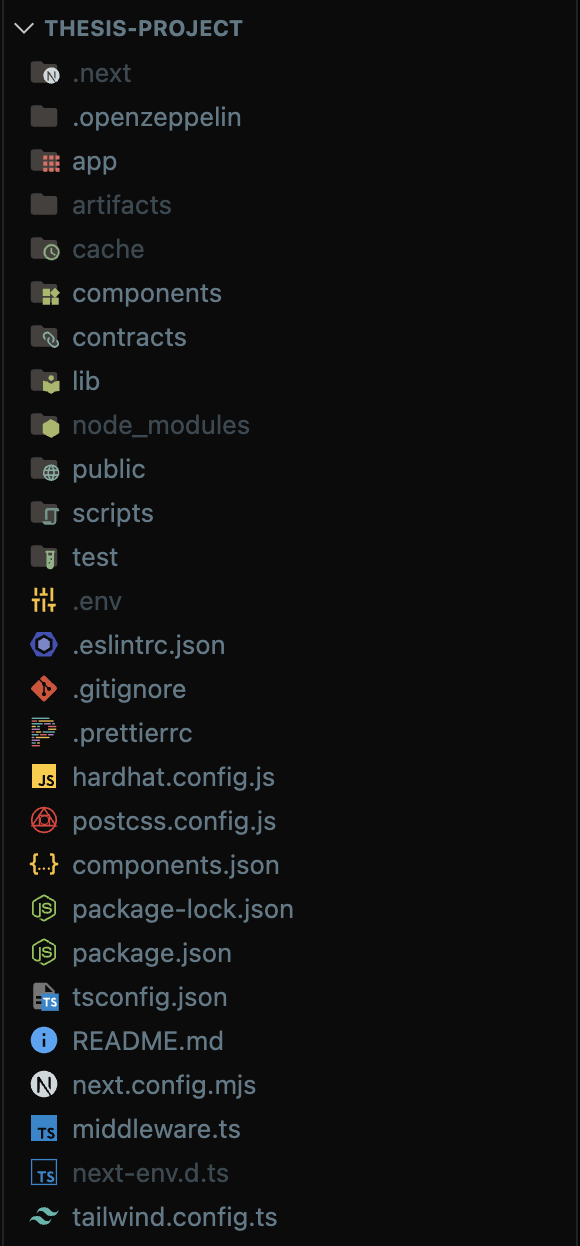
\includegraphics[scale=0.3]{src/images/folder-structure.png}
	\caption{Фолдерийн бүтэц}
\end{figure}

\begin{itemize}
	\item \textbf{components} - React компонентууд
	\item \textbf{lib} - Хэрэглэгчийн талын шаардлагатай код туслах функцууд
	\item \textbf{app} - NextJS дээрх хуудаснууд
	\item \textbf{public} - Статик зураг, файлууд
	\item \textbf{scripts} - Ухаалаг гэрээний хөгжүүлэлтийн холбоотой  javascript файлууд
	\item \textbf{contracts} - Ухаалаг гэрээний файлууд
\end{itemize}

\subsection{Ухаалаг гэрээн хөгжүүлэлт}
Миний төсөл нэг ухаалаг гэрээнээс бүтнэ.
Уг ухаалаг гэрээ нь цахим файлууд болон тэдгээртэй холбоотой лицензүүдийг төлөөлдөг Файл ба Лиценз гэсэн хоёр бүтцийг тодорхойлсон. Эдгээр бүтэц нь файлын ID, эзэмшигчийн хаяг, файлын нэр, тайлбар, ангилал, файлын хэш, үүсгэсэн хугацааны  зэрэг атрибутуудыг агуулна. Мөн дараах функцуудтэй:

\begin{itemize}
	\item \textbf{createFile}
	\item \textbf{issueLicense}
	\item \textbf{getAllPublicFiles}
	\item \textbf{getAllUserFiles}
	\item \textbf{getAllUserLicenses}
	\item \textbf{validateLicense}
	\item \textbf{getPublicFileById}
	\item \textbf{getMarketplaceFiles}
	\item \textbf{generateUniqueLicense}
\end{itemize}

\lstinputlisting[language=Java, caption=Ухаалаг гэрээ,basicstyle=\linespread{0.8}\ttfamily,frame=single]{src/code/smart-contract.sol}

\subsection{Ухаалаг гэрээг блокчейнд байршуулах}
\lstinputlisting[caption=Ухаалаг гэрээ,basicstyle=\linespread{0.8}\ttfamily,frame=single]{src/code/deploy.js}

\subsection{Хэрэглэгч талын хөгжүүлэлт (Front-end)}
Уг код нь хэрэглэгчийн оруулах цахим баримт бичгийн мэдээллийг блокчейнд бичнэ.
\lstinputlisting[ caption=,basicstyle=\linespread{0.8}\ttfamily,frame=single]{src/code/writeFile.ts}

Энэ функц нь хэрэглэгчийн оруулсан баримт бичгийг IPFS-д байршуулна.
\lstinputlisting[caption=Файл IPFS-д  байршуулах,basicstyle=\linespread{0.8}\ttfamily,frame=single]{src/code/uploadIpfs.ts}

Уг код нь хэрэглэгчийн оруулсан цахим баримт бичгүүдийн мэдээллийг блокчейнээс уншина.
\lstinputlisting[caption=,basicstyle=\linespread{0.8}\ttfamily,frame=single]{src/code/getUserFiles.ts}


\pagebreak
\subsection{Үр дүн}
Төслийн практик ажлын үр дүнд бүтээгдсэн  системийн интерфейс дараах байдлаар харагдана.
\begin{figure}[h!]
	\centering
	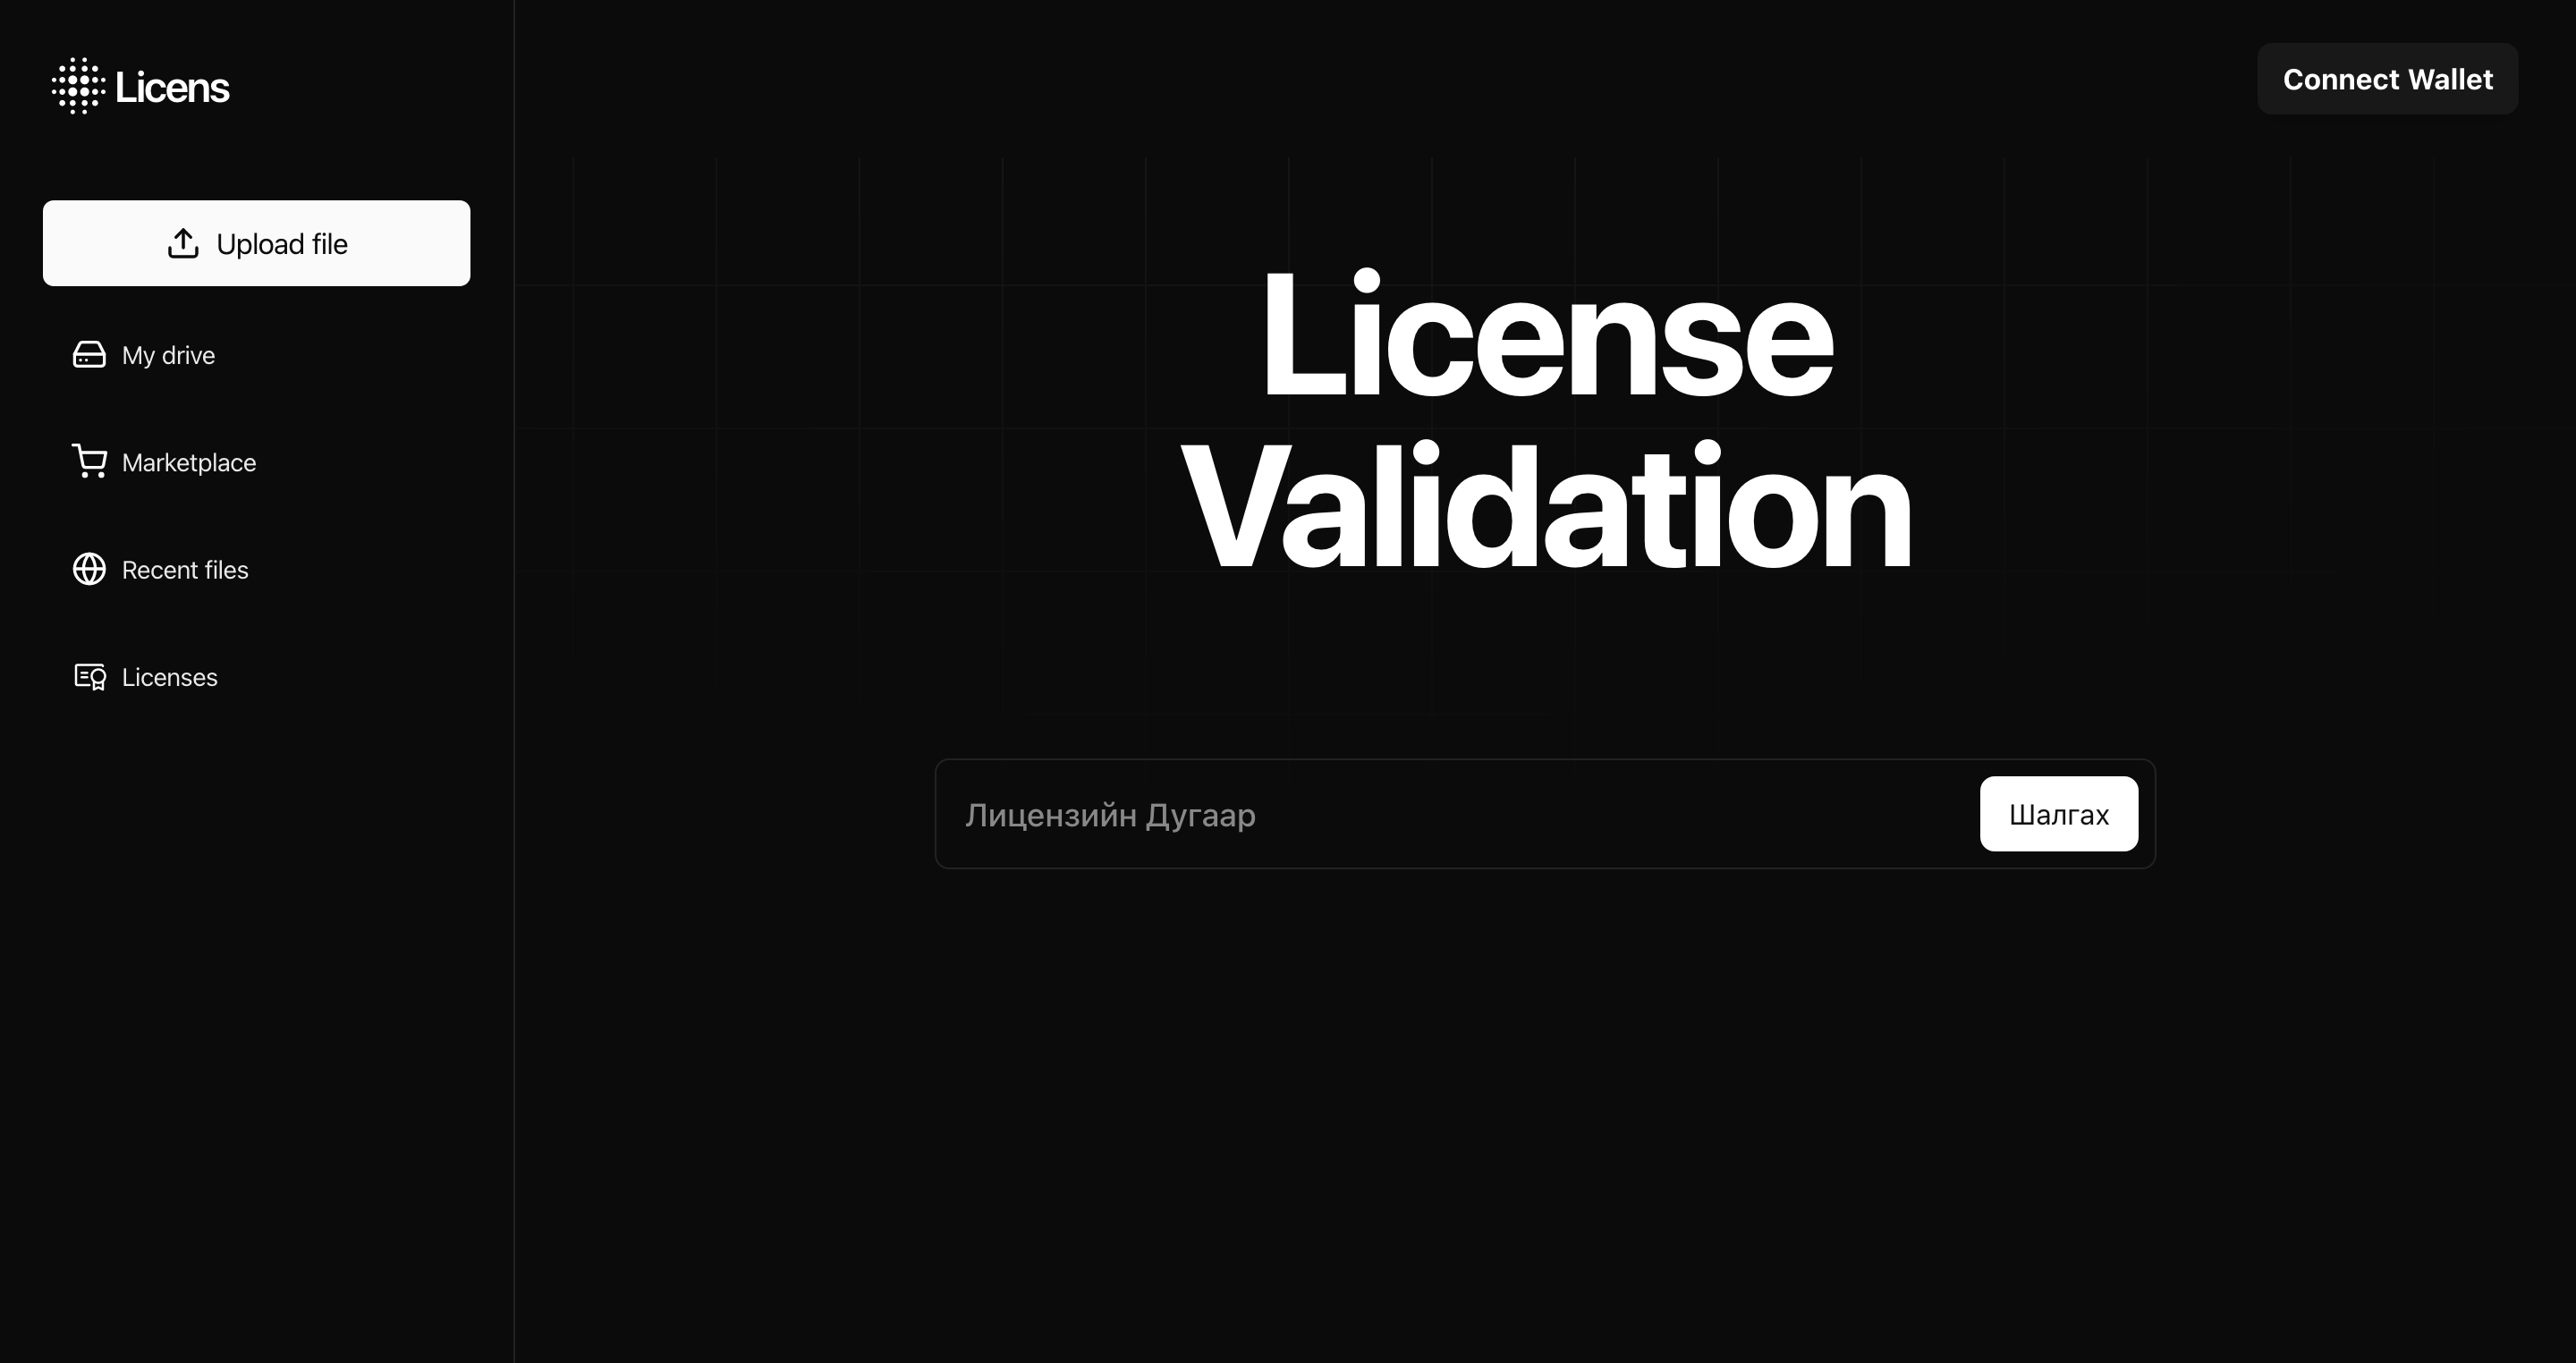
\includegraphics[scale=0.155]{src/images/homepage.png}
	\caption{Нүүр хуудас}
\end{figure}

\begin{figure}[h!]
	\centering
	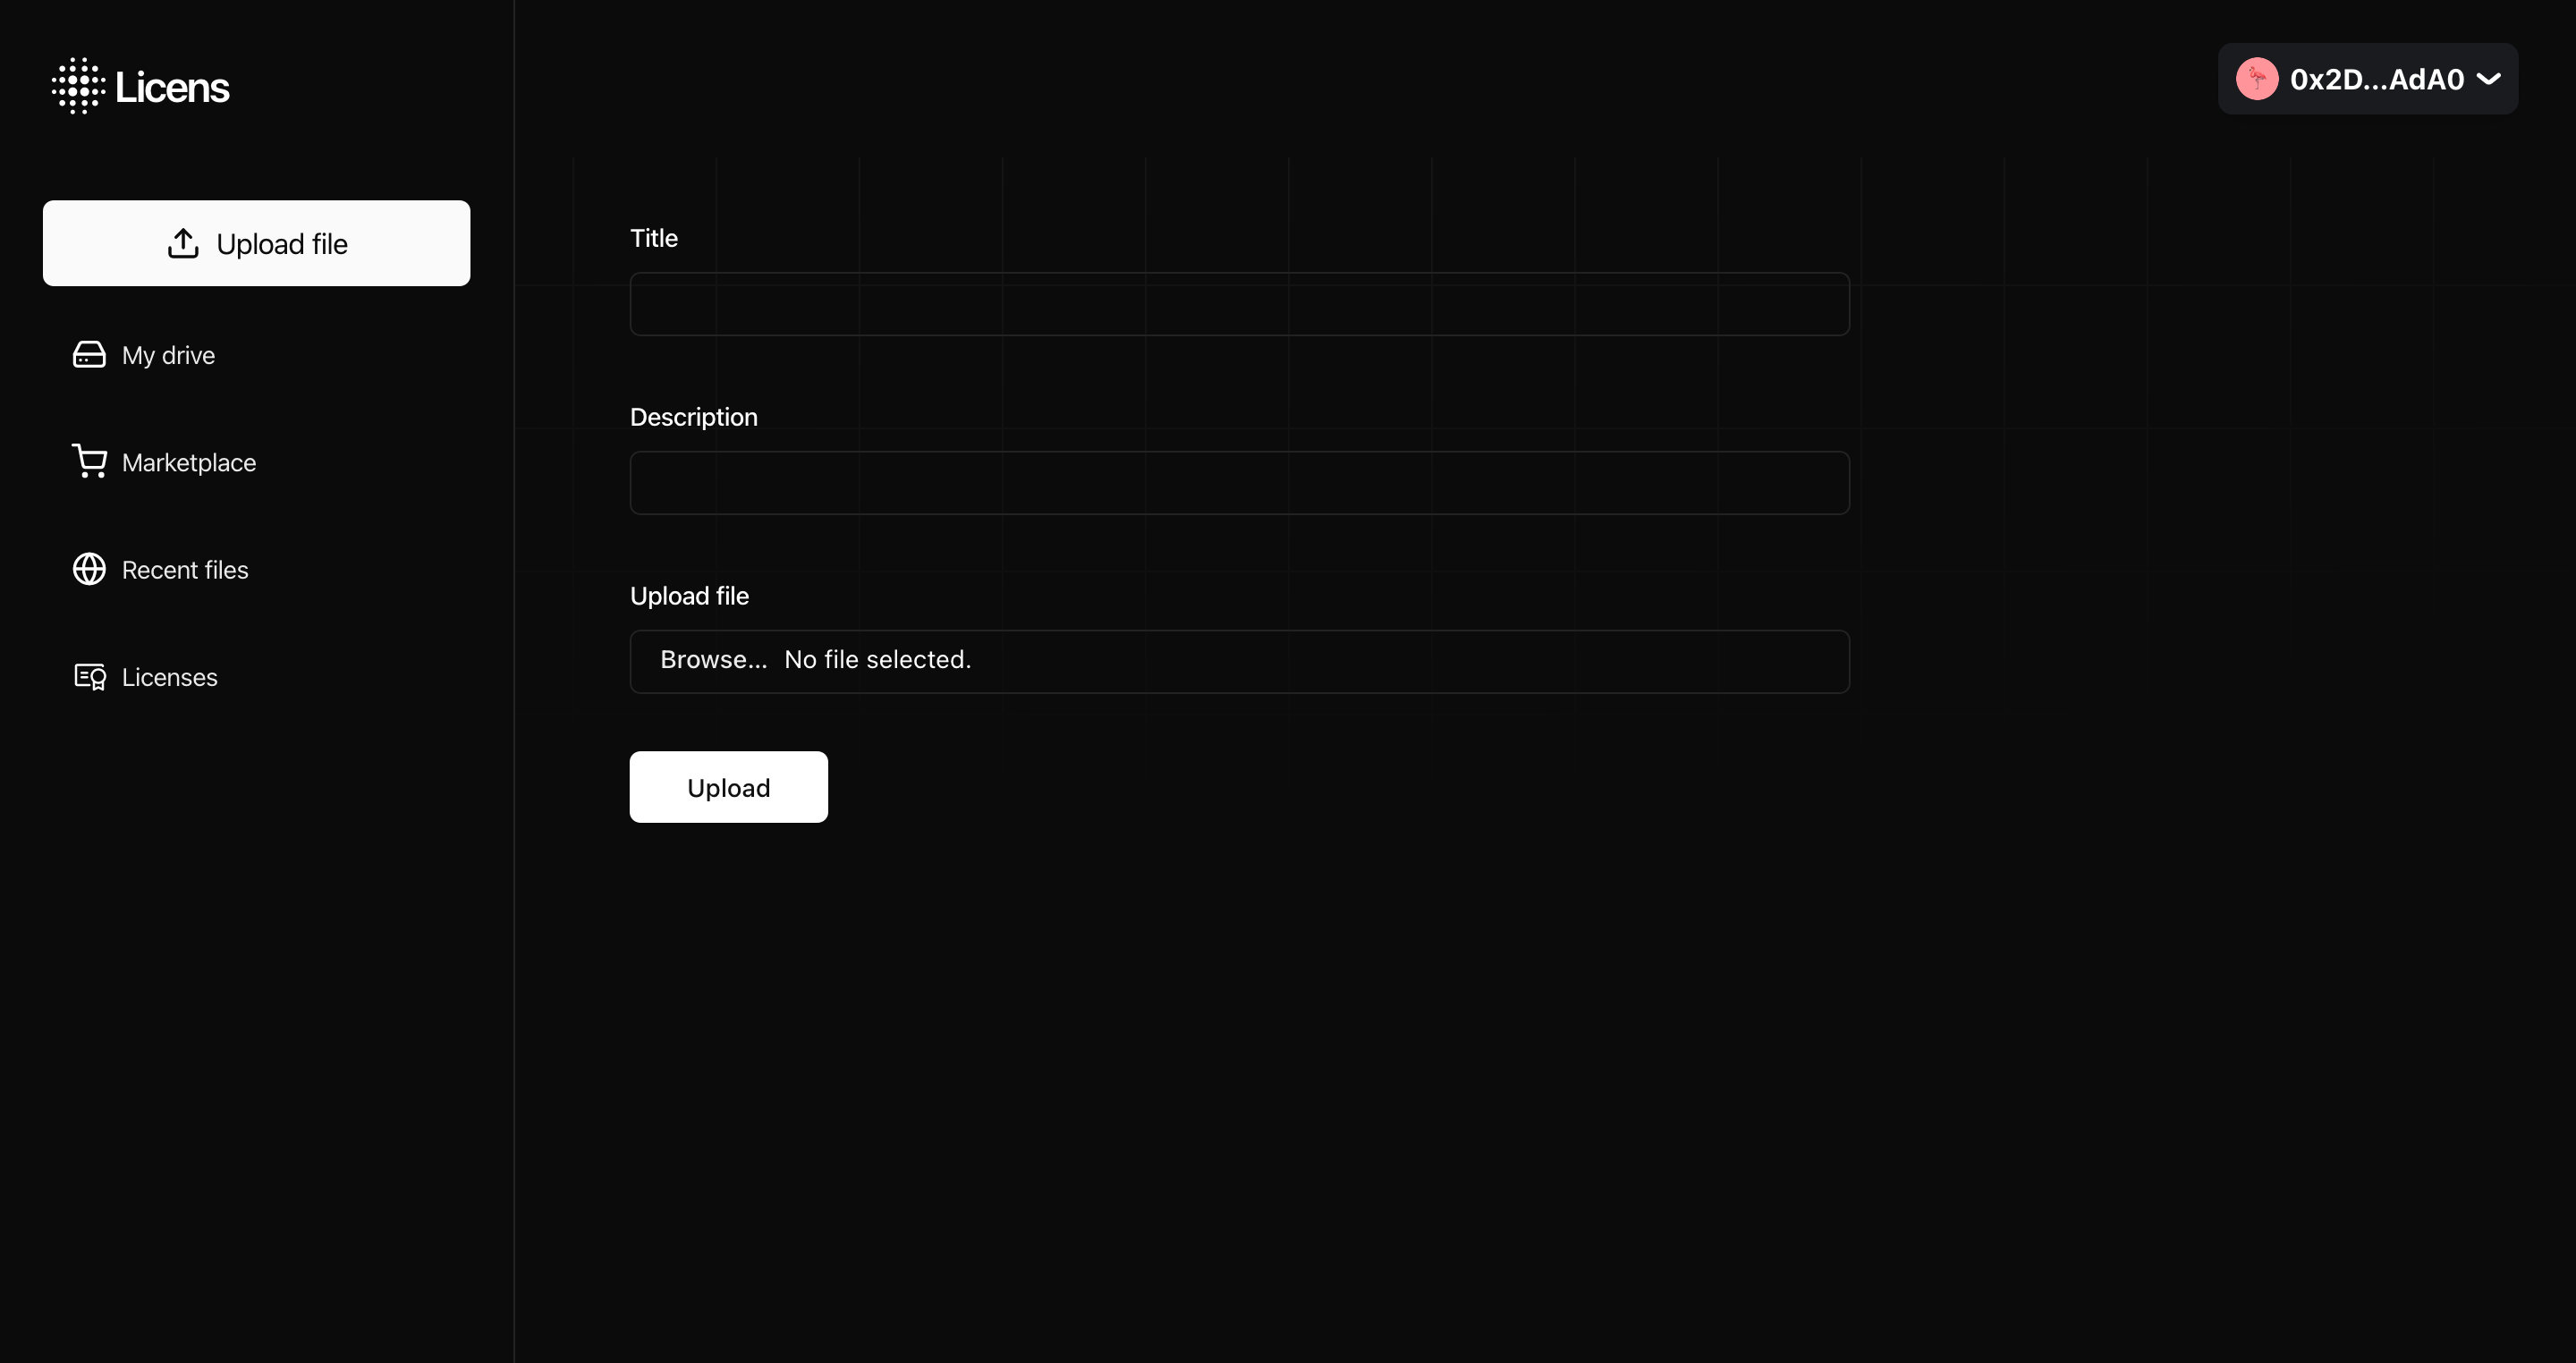
\includegraphics[scale=0.155]{src/images/upload-page.png}
	\caption{Цахим бичиг баримт оруулах}
\end{figure}

\begin{figure}[h!]
	\centering
	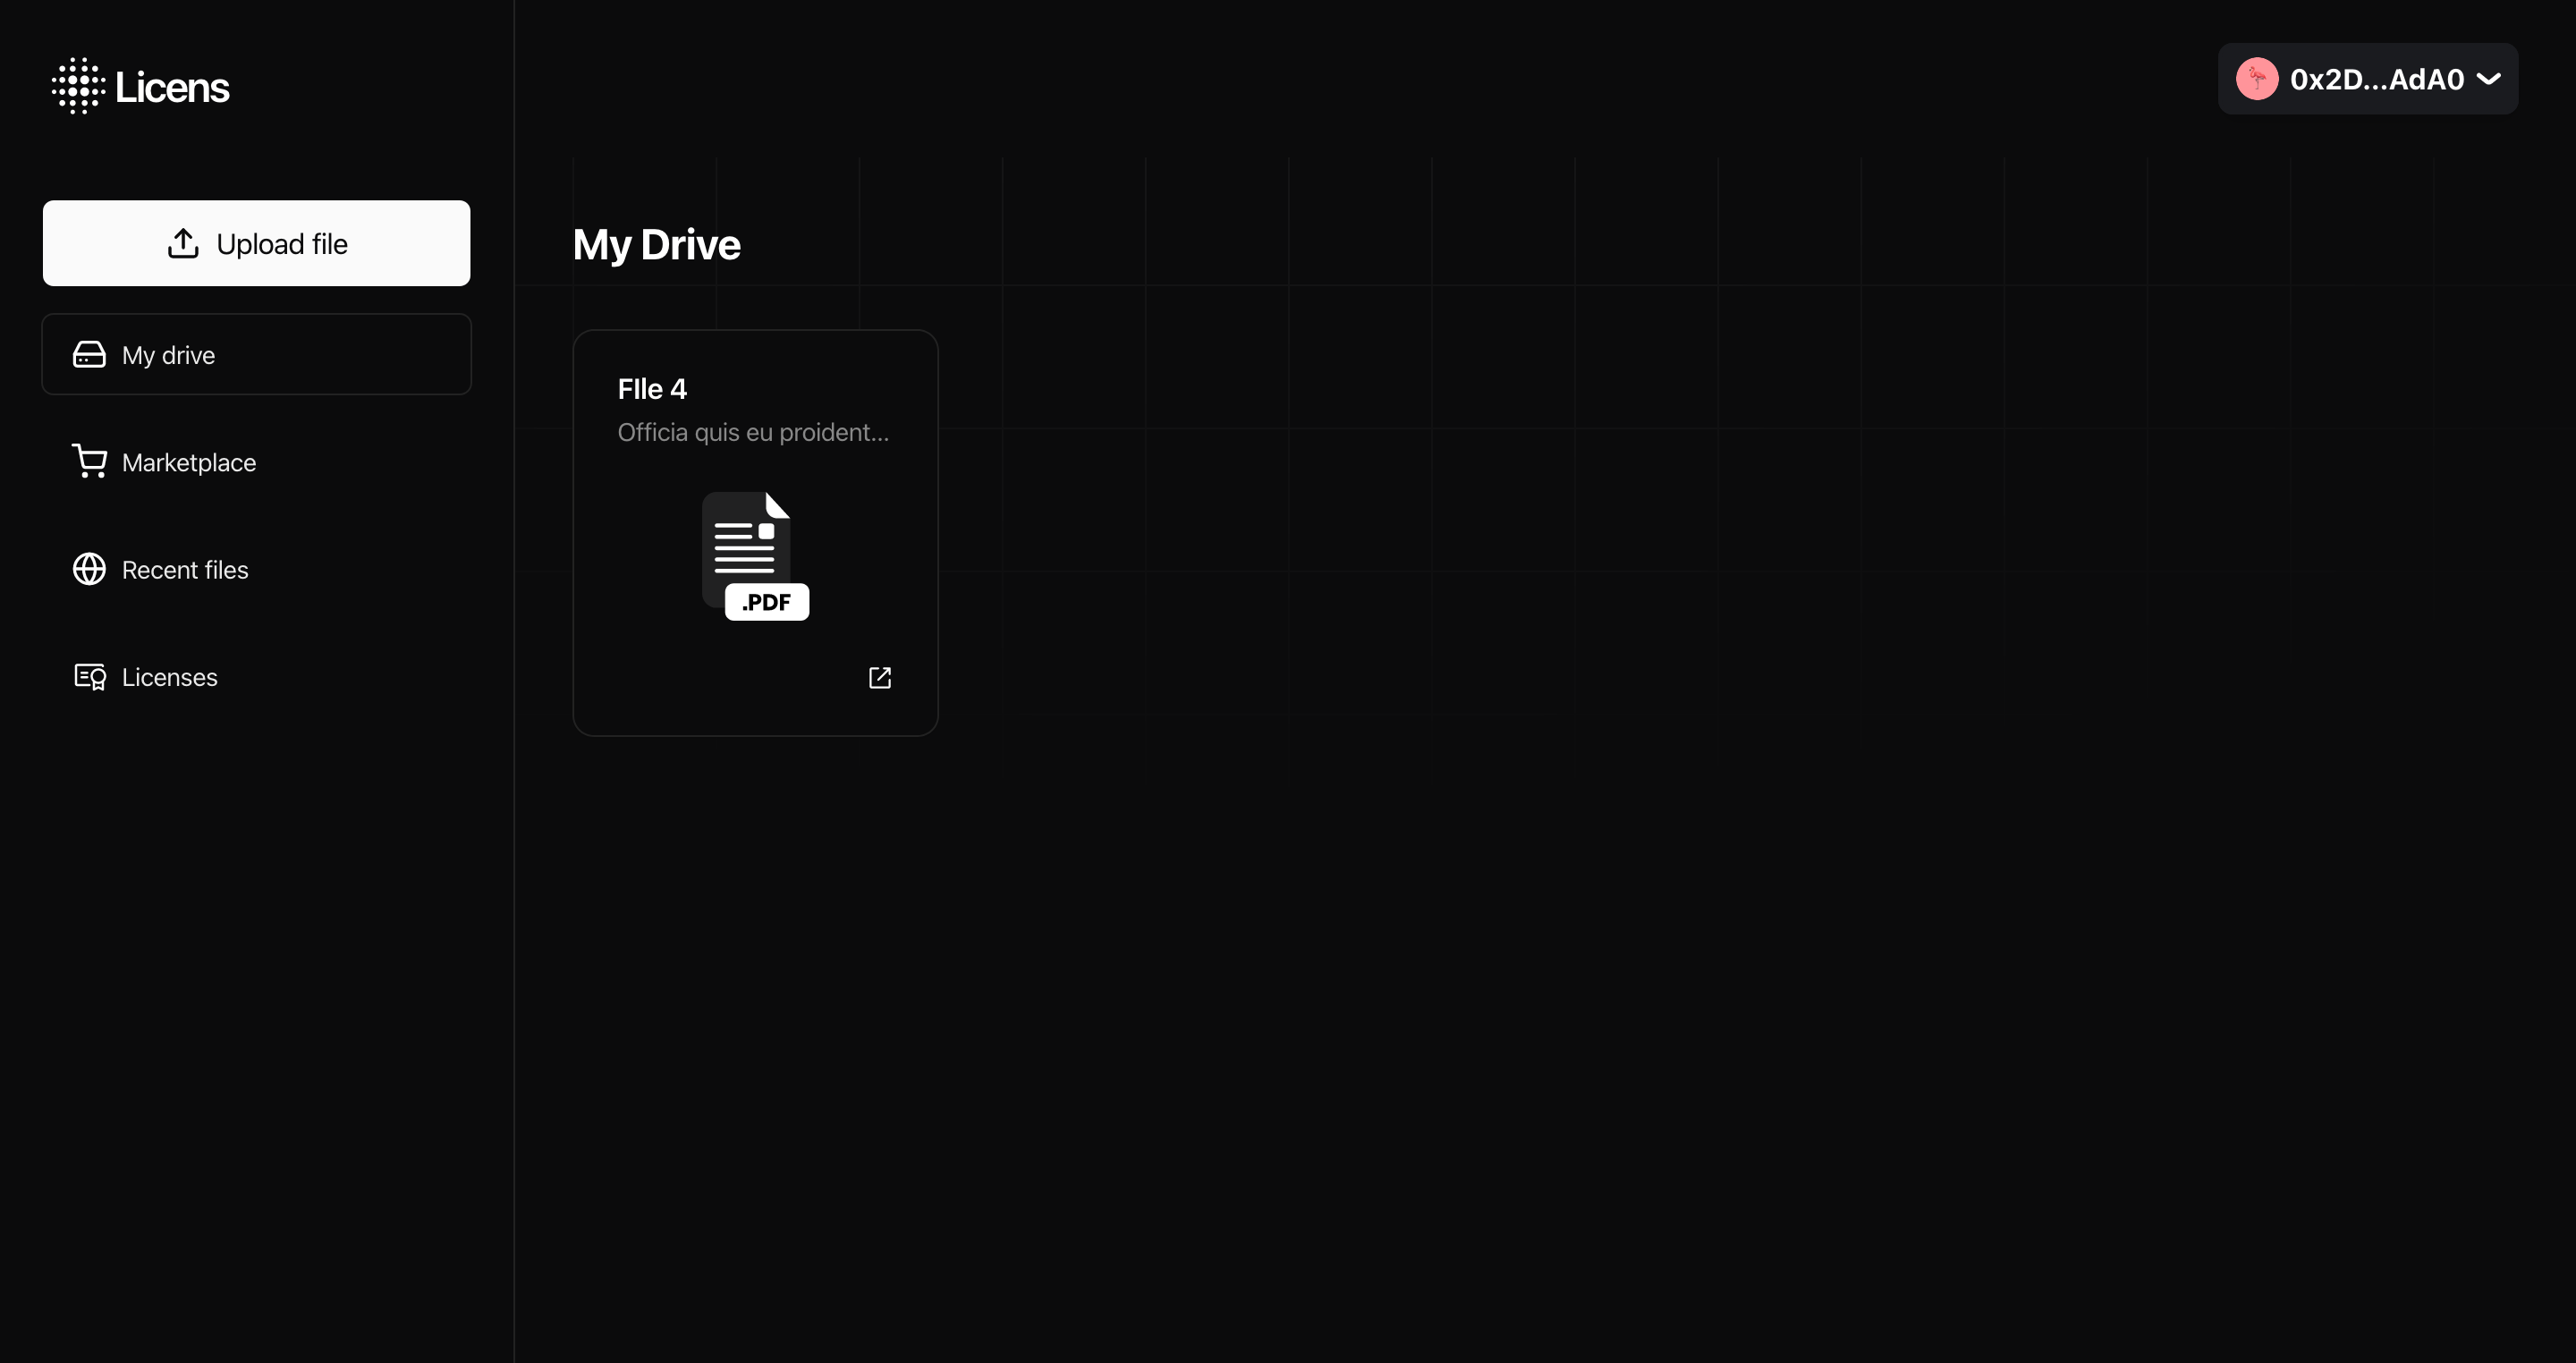
\includegraphics[scale=0.165]{src/images/drive-page.png}
	\caption{}
\end{figure}

\begin{figure}[h!]
	\centering
	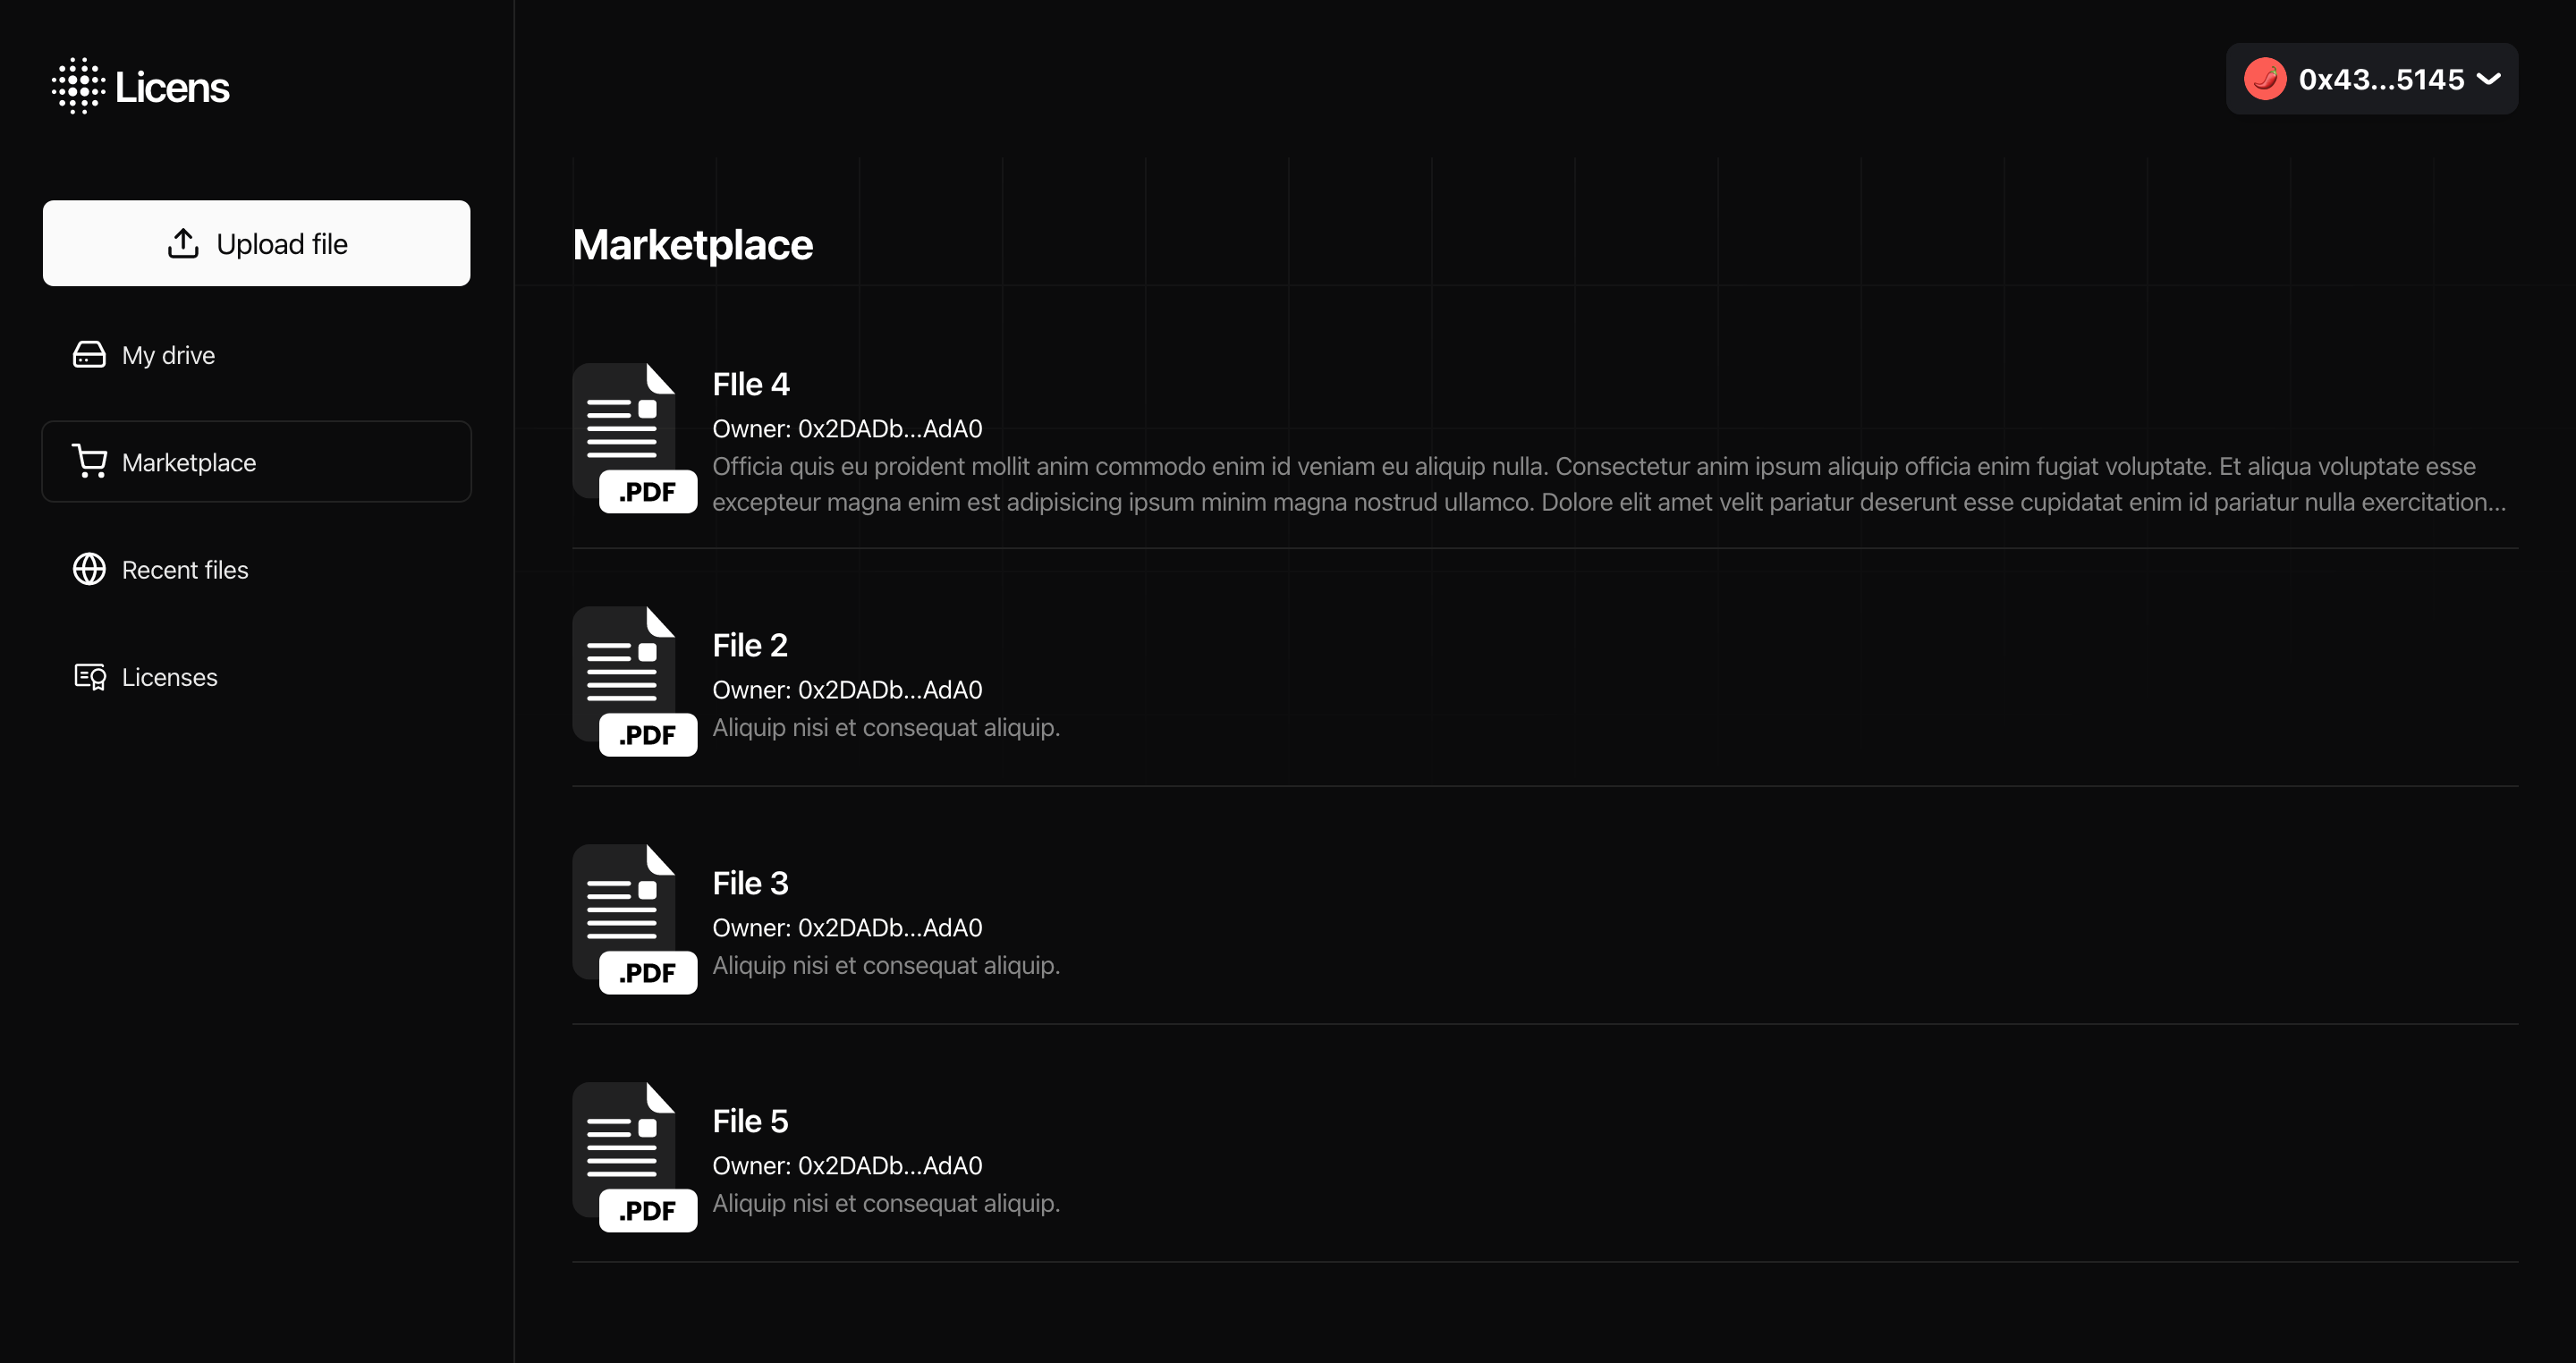
\includegraphics[scale=0.165]{src/images/marketplace-page.png}
	\caption{}
\end{figure}

\begin{figure}[h!]
	\centering
	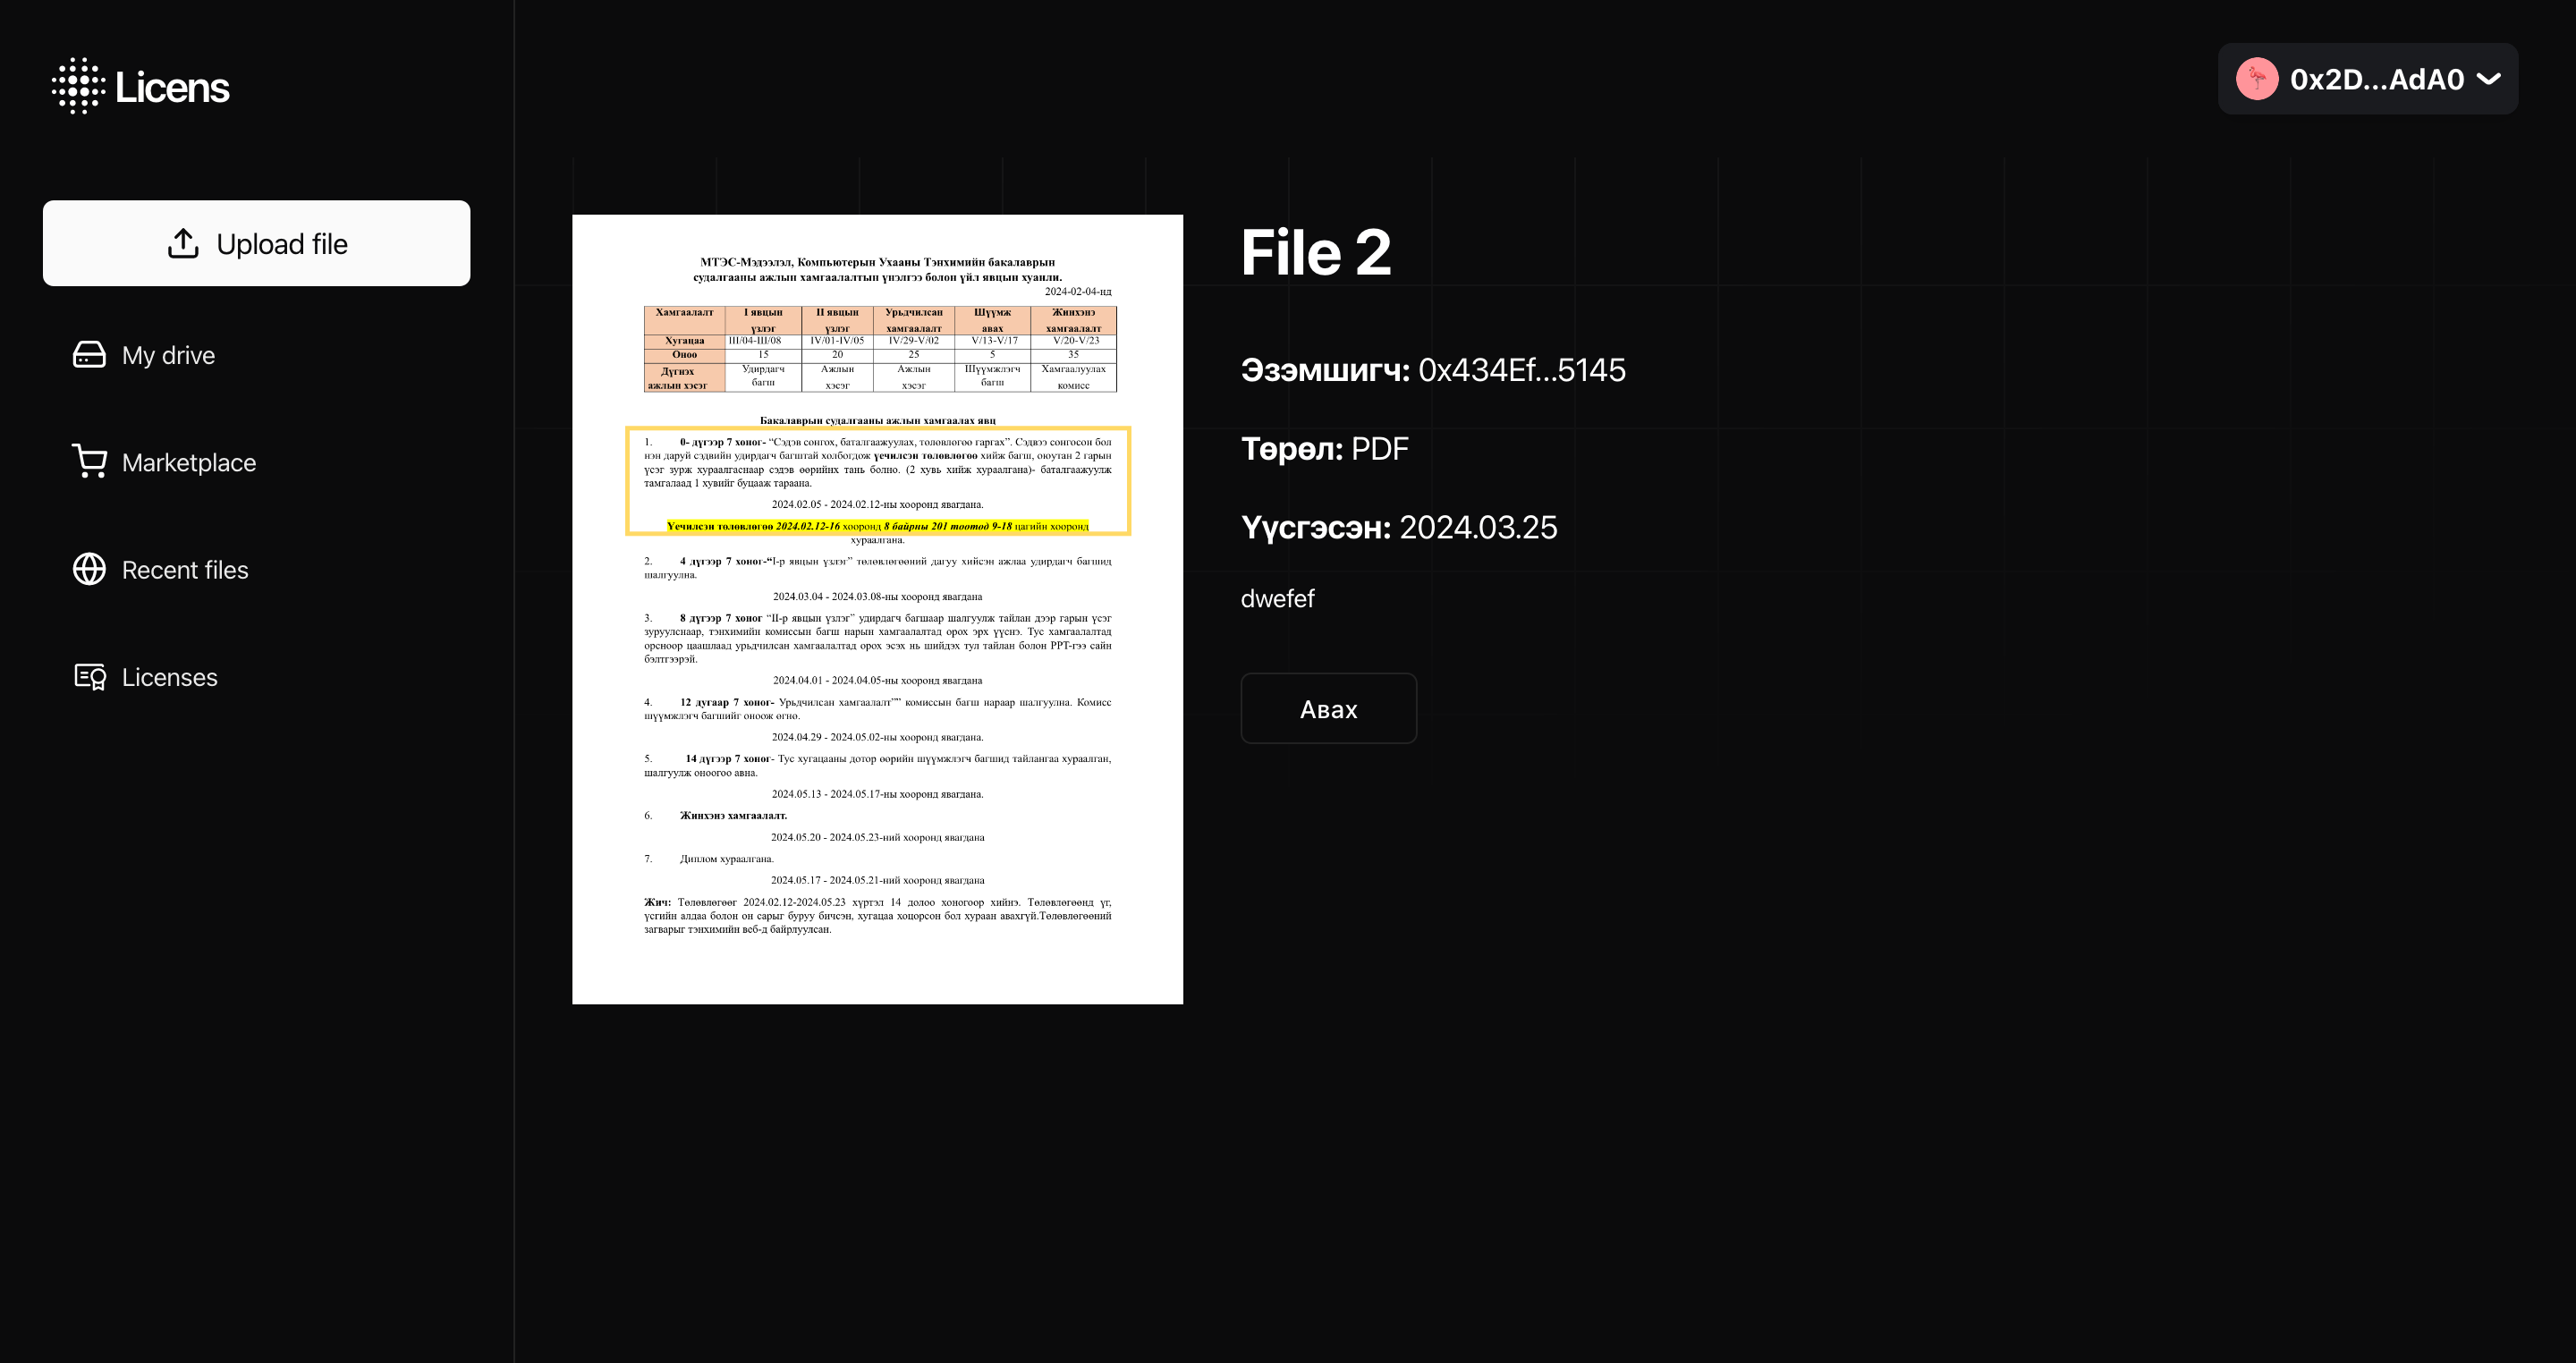
\includegraphics[scale=0.165]{src/images/file-page.png}
	\caption{}
\end{figure}